\documentclass[11pt]{article} 

%\documentclass[paper=a4,fontsize=11pt]{scrartcl}	 			% KOMA-article class
							
%\usepackage[english]{babel}								% English language/hyphenation
%\usepackage[protrusion=true,expansion=true]{microtype}		% Better typography
\usepackage{amsmath,amsfonts,amsthm}					% Math packages
\usepackage[pdftex]{graphicx}								% Enable pdflatex
\usepackage[svgnames]{xcolor}							% Colors by their 'svgnames'
\usepackage{geometry}
	\textheight=700px									% Saving trees ;-) 
\usepackage{url}										% Clickable URL's
\usepackage{wrapfig}									% Wrap text along figures


\frenchspacing									% Better looking spacings after periods
%\pagestyle{empty}								% No pagenumbers/headers/footers
%\usepackage{bbding}									% Symbols


% ------- Enable UTF8 characters ------- %
%\usepackage[utf8]{inputenc}
\usepackage[english]{babel}

\usepackage{listings}
\usepackage{color}

%\usepackage{pdfpages}

% ------------ Code Listing ------------- %

\definecolor{dkgreen}{rgb}{0,0.6,0}
\definecolor{gray}{rgb}{0.5,0.5,0.5}
\definecolor{mauve}{rgb}{0.58,0,0.82}

\lstset{frame=false,
  language=C++,
  aboveskip=3mm,
  belowskip=3mm,
  showstringspaces=false,
  columns=flexible,
  basicstyle={\small\ttfamily},
  numbers=none,
  numberstyle=\tiny\color{gray},
  keywordstyle=\color{blue},
  commentstyle=\color{dkgreen},
  stringstyle=\color{mauve},
  breaklines=true,
  breakatwhitespace=true,
  tabsize=3,
  moredelim=**[is][\color{mauve}]{@}{@},
}

% ------- Page layout ------- %
\usepackage{fullpage}
\usepackage{hyperref} % clickable references
\hypersetup{
    colorlinks,
    citecolor=black,
    filecolor=black,
    linkcolor=black,
    urlcolor=black
}
\usepackage{multicol}
\setlength{\columnsep}{1cm}

% ------- Images ------- %
\usepackage{graphicx}
\usepackage{caption}
\usepackage{float}
\usepackage{subcaption}
\DeclareCaptionFont{gray}{\color{gray}}
\captionsetup{textfont={footnotesize,sc,gray},font={footnotesize,sc,gray}}
\usepackage{blindtext}

% Test

\usepackage{tikz}
\usetikzlibrary{shapes,arrows,shadows}
\newcommand{\mx}[1]{\mathbf{\bm{#1}}} % Matrix command
\newcommand{\vc}[1]{\mathbf{\bm{#1}}} % Vector command

\usetikzlibrary{arrows}


\title{Elektriske Maskiner}


\begin{document}

\begin{titlepage}
\begin{center}


\textsc{\LARGE University of Southern Denmark}\\[1.5cm]
\textsc{\Large RoVi1 -- Introduction to Robotics and Computer Vision}\\[0.5cm]
\vfill
\hrule ~\\[0.3cm]
{ \huge \bfseries Mandatory Exercise 2\\[0.4cm] }
\hrule ~\\[1.5cm]
\vfill

% Author and supervisor
\begin{minipage}[t]{7.9cm}
\begin{flushleft} \large
\emph{by:}\\
Keerthikan Ratnarajah  \\
kerat12@student.sdu.dk \\
Jes Grydholdt Jepsen   \\
jejep12@student.sdu.dk 
\end{flushleft}
\end{minipage}
\begin{minipage}[t]{7.9cm}
\begin{flushright} \large

\end{flushright}
\end{minipage}

\vspace{1.2cm}
Dato: \today


\end{center}
\end{titlepage}

\tableofcontents

\newpage
\section{Implementation and theory}
This project considers the robotic scene \textit{“Kr16WallWorkCell”}, where a program is developed for making a robotic pick and place operation. The robot arm picks up the object using the joint configuration $q_{pick}$ and place the object at the joint configuration $q_{place}$ .
\begin{eqnarray*}
q_{pick} &=& (-3.142,-0.827,-3.002,-3.143,0.099,-1.573) [rad] \\
q_{place} &=& (1.571,0.006,0.030,0.153,0.762,4.490) [rad]
\end{eqnarray*}
The RRT-connect is used for finding a collision free path between the two joint configurations. The solution consists of two parts; a C++ project and a LUA script. The C++ project is a modified version of the “pathplanner.cpp”-file which includes RobWork (RW) and makes a RRT-planner in RW, and the LUA script is executed in RobWorkStudio (RWS) to simulate the results of the RRT-planner, and in that way check if the robot arm or the bottle collides with any of the obstacles in the workspace. In both programs is the grasp of the bottle taken into account in the code, and especially in the path planner to ensure that is not only makes a collision free path for the robot arm, but also for the bottle when it is attached. In order to do this in the C++ project, the frame of the bottle is added to the robot arm’s end effector. One way to this in RW is by first defining the workcell, the robot arm and the item to grasp with the robot arm
\begin{lstlisting}
	// Set the names
    const string wcFile = "../Kr16WallWorkCell/Scene.wc.xml";
    const string deviceName = "KukaKr16";
    const string bottle = "Bottle";
    
    // Set from and to
    Q from(6,-3.142,-0.827,-3.002,-3.143,0.099,-1.573);
    Q to(6,1.571,0.006,0.030,0.153,0.762,4.490);
    
    WorkCell::Ptr wc = WorkCellLoader::Factory::load(wcFile);
    
    // Set the device of the robot arm
    Device::Ptr device = wc->findDevice(deviceName);
	
	// Find the frame of the item to grasp
    rw::kinematics::Frame *deviceB = wc->findFrame(bottle);
    
    rw::kinematics::State state = wc->getDefaultState();
    
    device->setQ(from, state);
\end{lstlisting}
\noindent and attach the bottle by adding the bottles frame on the end of the robot arms frame
\begin{lstlisting}
    Kinematics::gripFrame(deviceB,device->getEnd(),state);
\end{lstlisting}

\begin{lstlisting}

\end{lstlisting}

\newpage
\subsection{RRT-connect}
RRT-connect path planner basically builds two trees; one from the source point and one from the destination point with a given step stepsize.  The algorithm randomly starts growing the two trees towards each other, both from the source and the destination, and a path is found when the two trees connect. Advantages of this algorithm is that it will always find a path if possible, but the disadvantages is that the computational time is highly variable because of the random factor, and the found path is not repeatable or predictable.

\begin{figure}[H]
\centering
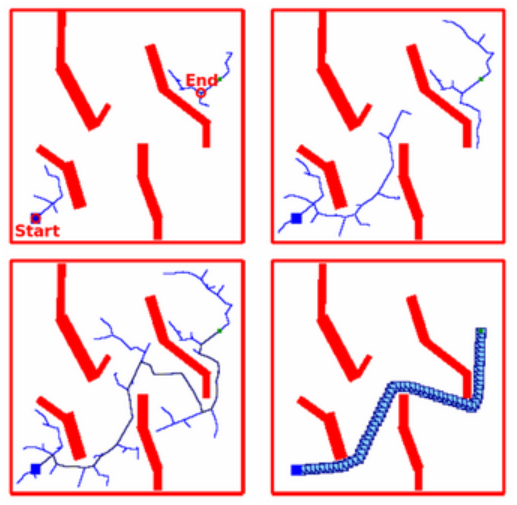
\includegraphics[scale=0.5]{img/Selection_050.png}
\caption{Illustration of the RRT-connect algorithm}
\label{fig::rrt}
\end{figure}

\noindent The length of each connection the algorithm grows the trees with is called epsilon. The parameter epsilon determines both the speed and precision of the path planner. The smaller epsilon is, the more accurate is the planner, but conversely will the time it takes to find the path between the source and the destination increase. To optimize the performance with respect to the path length and the search time a good estimate for this project is needed to be found. In order to do that, some statistics of different test results has been made. These statistics are necessary because the RRT-connect is a probabilistic method, which means that the solution between the source and the destination different each time, and therefore will the computation time also vary. In the C++ project the path planning is done by 
\begin{lstlisting}
	CollisionDetector detector(wc, ProximityStrategyFactory::makeDefaultCollisionStrategy());
    PlannerConstraint constraint = PlannerConstraint::make(&detector,device,state);

    QSampler::Ptr sampler = QSampler::makeConstrained(QSampler::makeUniform(device),constraint.getQConstraintPtr());
    QMetric::Ptr metric = MetricFactory::makeEuclidean<Q>();
    QToQPlanner::Ptr planner = RRTPlanner::makeQToQPlanner(constraint, sampler, metric, extend, RRTPlanner::RRTConnect);

    QPath path;
    planner->query(from,to,path,MAXTIME);
\end{lstlisting}
and in order to get each joint configuration, the following code is used for iterating through them
\begin{lstlisting}
for (QPath::iterator it = path.begin(); it < path.end(); it++) {
        cout << *it << endl;
    }
\end{lstlisting}

\section{Data acquisition}
The data to estimate a proper epsilon value was acquired using the the cpp file  pathplanner.cpp.    The code does the pathplanning from one joint configuration ($Q_{from}$) to another joint configuration ($Q_{to}$) given a workcell in Robwork.   To make the Robot grasp the bottle were these line added to the code.
\begin{lstlisting}
const string bottle = "Bottle"; 	
\end{lstlisting}
Defines the name of object going to be grasped. 
\begin{lstlisting}
rw::kinematics::Frame *deviceB = wc->findFrame(bottle);
\end{lstlisting}
Finds the frame “bottle” defined in the workcell wc.
\begin{lstlisting}
Kinematics::gripFrame(deviceB,device->getEnd(),state);
\end{lstlisting}
Adds the frame bottle at the end of the device (being the robot). which is then added to the state consisting of the tree structure. The tree structure consist of the structure of how the workcell is is divided.

\begin{figure}[H]
\centering
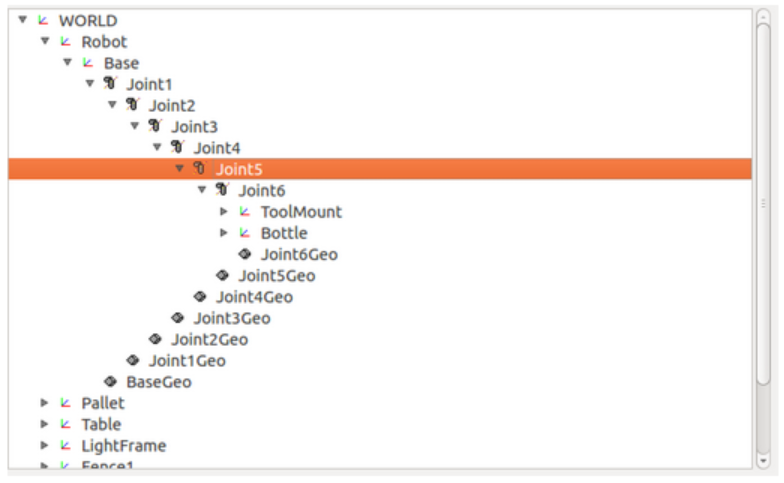
\includegraphics[scale=0.4]{img/Selection_051.png}
\caption{Illustration of the tree structure}
\label{fig::rrt}
\end{figure}

At which gripFrame add the bottle at the end of Joint6 being the same as the ToolMount.\\[0.2cm] 

\noindent These were the addition made to the code. The code itself print the different joint configuration given different epsilon values (given as extend).

\begin{lstlisting}
double extend = 0.5;
\end{lstlisting}

\noindent And prints the values here. 
\begin{lstlisting}
for (QPath::iterator it = path.begin(); it < path.end(); it++) {
        //cout << "set" << *it << endl;
    }
\end{lstlisting}

\begin{lstlisting}
setQ{-3.142, -0.827, -3.002, -3.143, 0.099, -1.573}
setQ{-3.11042, -0.806822, -2.99561, -3.12343, 0.0832693, -1.5524}
setQ{-3.09549, -0.798532, -2.99925, -3.08662, 0.0940422, -1.52549}
setQ{-3.07207, -0.789749, -3.00322, -3.05822, 0.107558, -1.55498}
setQ{-3.07072, -0.790792, -3.00119, -3.01273, 0.112007, -1.57507}
setQ{-3.03991, -0.783541, -2.99792, -3.02226, 0.0910588, -1.60602}
setQ{-3.01517, -0.776191, -3.00139, -2.99158, 0.0814082, -1.63407}
setQ{-3.00403, -0.770283, -3.00218, -3.00624, 0.0988269, -1.67676}
setQ{-3.00131, -0.7709, -2.99906, -2.96079, 0.094911, -1.69681}
setQ{-2.96601, -0.768664, -2.99227, -2.93546, 0.0971116, -1.72039}
setQ{-2.92738, -0.757517, -2.96939, -2.93405, 0.0911586, -1.73837}
setQ{-2.91543, -0.756617, -2.96207, -2.89046, 0.0977794, -1.75731}
setQ{-2.87822, -0.745384, -2.94019, -2.87864, 0.0896049, -1.77475}
...
setQ{1.571, 0.006, 0.03, 0.153, 0.762, 4.49}
\end{lstlisting}


\section{Data processing}
To acquire the optimal value of epsilon for the pathplanning between $Q_{pick}$ to $Q_{place}$,  the maximum needed change in joint configuration had to be computed. Each joint is capable of turning 2$\pi$ Rad, making the search for an optimal epsilon limited to the range of 0 - 2$\pi$
 
 
\noindent To find the optimal value, were different paths computed using different epsilon values with an stepsize of 0.01.  At each step was the path length, movement time.   Which led to this graph, each step was computed 10 times, and the average of each value plotted is plotted in Figure \ref{fig::graph} .\\[0.2cm]

\begin{figure}[H]
\hspace{-3.5cm}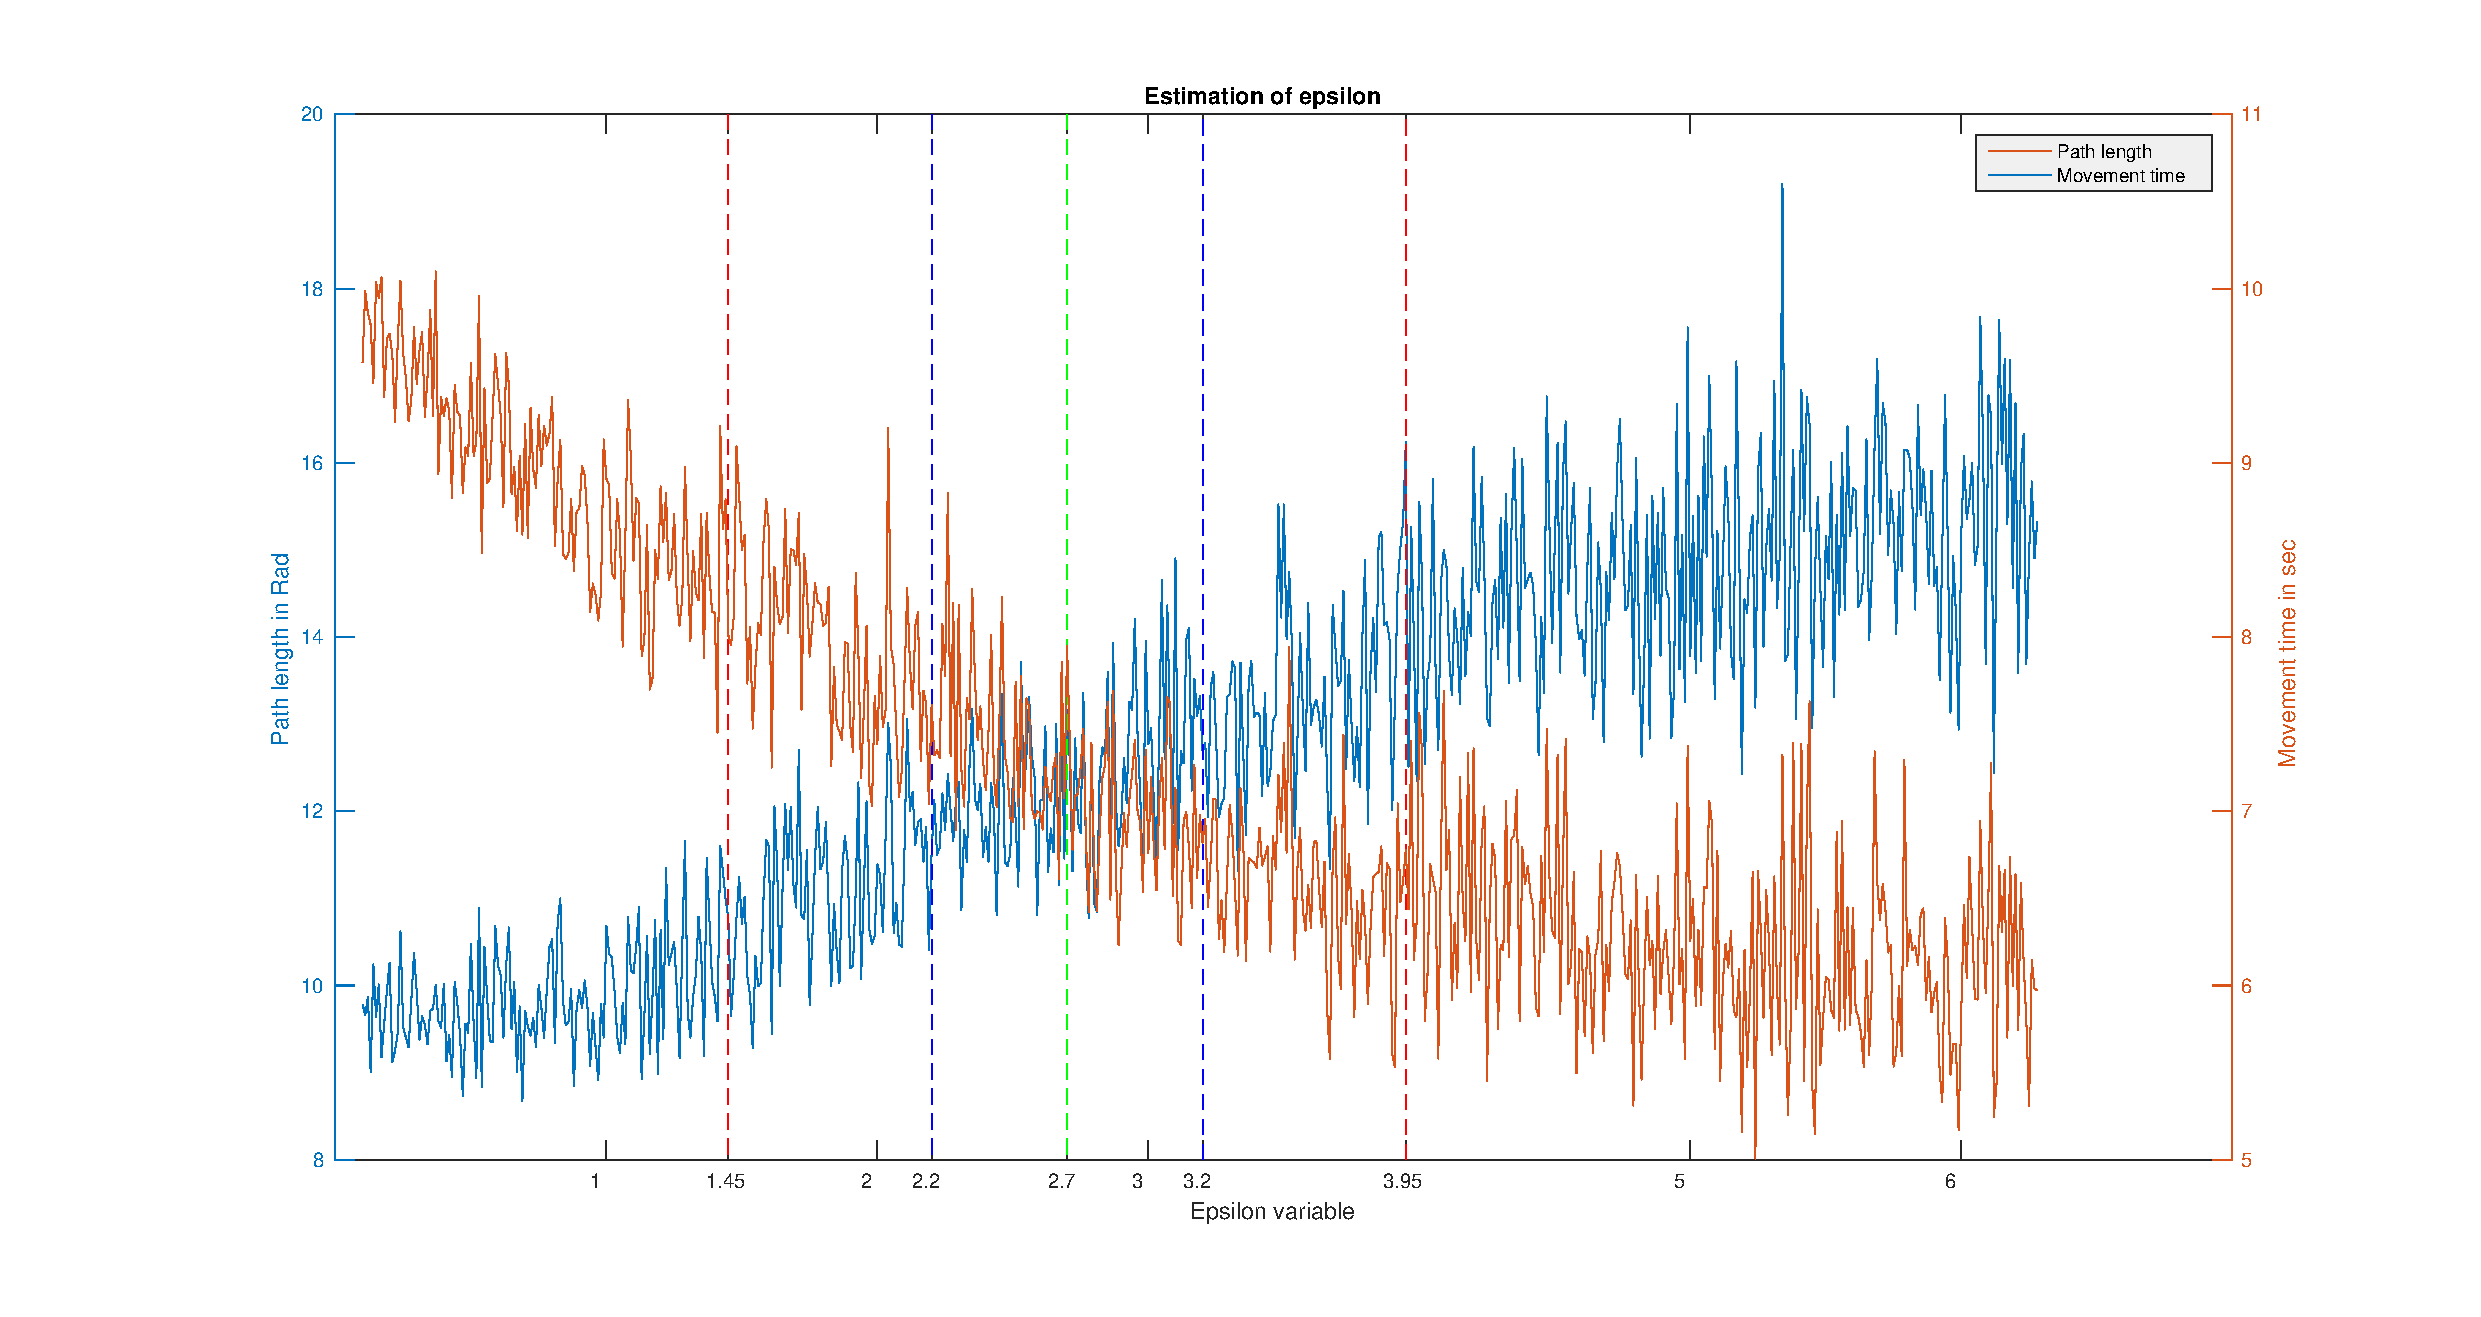
\includegraphics[scale=0.55]{img/graph.eps}
\caption{Comparison of the path length and the time it takes to perform the movement}
\label{fig::graph}
\end{figure}

\noindent Figure \ref{fig::graph}  compares the path length  to time it takes to perform the movement.  It can clearly be seen that  that around $\epsilon = 2.7$  both the graphs intersect each other, showing the optimal length and movement time  for this movement. 
\\

The graph shows that both graph intersect each other at $\epsilon = 2.7$ making it the optimal choice for this movement.  The graph also show a correlation between these parameter.  The pathlength increases for higher of $\epsilon$ due, which would occur due to overshoot, and vice versa a higher movement time for a low epsilon, but a low pathlength, as the robot will be able to move in small steps, ensuring that it still on the right track. 
%Add conclussion 


\newpage
\section{Conclusion}
A program that could make a robotic pick and place operation between two joint configurations was successfully made.\\[0.2cm]


\noindent For finding a collision free path between the two joint configurations was the RRT-connect algorithm implemented in a C++ project, and the found path was put in a LUA script and run in RobWorkStudio for testing if the KukaKr16 collides with any of the surroundings in the workcell. The best value for the parameter epsilon was found by testing the implementation with various values of epsilon. By plotting and comparing the values for the planning time and path size for the different epsilon values, an estimation of the best epsilon value for this project was found to be between 2.2 and 3.2.


\end{document}






















































